\documentclass{scrartcl}
\usepackage{amsmath, amssymb}
\usepackage{graphicx, float}
\usepackage{hyperref}
\usepackage[T1]{fontenc}
\begin{document}
\begin{center}
\textbf{\LARGE ACE Documentation}\\[2mm]
\textit{\Large Moritz Cygorek}
\end{center}
\section{Introduction}
This document describes how to use the C++ code ACE
for the solution of open quantum systems using the 
\emph{automated compression of environments} (ACE) method.
The article explaining the method can be found 
\href{https://doi.org/10.1038/s41567-022-01544-9}{here}.
%\href{https://arxiv.org/abs/2101.01653}{here}.

ACE enables numerically exact simulations of the dynamics of 
an open quantum systems described by the quantum Liouville equation
\begin{equation}
\frac{\partial}{\partial t} \rho=-\frac i\hbar [ H , \rho ] 
+\mathcal{L}_\textnormal{nonh.}[\rho]
\end{equation}
where the microscopic Hamiltonian 
%\begin{align}
\begin{equation}
H=H_S+H_E = H_S +\sum_{k=1}^{N_E} H_E^k,
\end{equation}
%\end{align}
is split up into system $H_S$ and environment Hamiltonians $H_E$.
The environment Hamiltonian $H_E$, 
which we define as also including the system-environment coupling, 
is assumed to be separable into $N_E$ independent modes $k$. 
%Throughout this document we will denote the dimension of the system Hilbert
%space by $N$ while the dimension of the $k$-th environment mode
%is $M^k$ (or simply $M$ if all $M^k$ are identical).
$\mathcal{L}_{nonh.}[\rho]=\mathcal{L}_S[\rho]+\mathcal{L}_E[\rho]
=\mathcal{L}_S[\rho]+\sum_k \mathcal{L}_E^k [\rho]$ 
denotes non-Hamiltonian contributions
to the dynamics such as Lindblad terms affecting the system 
and the environment.

The goal is to obtain the reduced system density matrix discretized on
a time grid $t_l = t_a + l \Delta t$ up to a given final time 
$t_n = t_a + n \Delta t = t_e$.
This can be done using the path integral expression
\begin{equation}
{\rho}_{\alpha_n}=
\sum_{\substack{\alpha_{n-1}\dots\alpha_0 \\
\tilde{\alpha}_n\dots\tilde{\alpha}_1}}
\mathcal{I}^{(\alpha_{n}\tilde{\alpha}_n)\dots(\alpha_1\tilde{\alpha}_1)}
\bigg(\prod_{l=1}^{n}
\mathcal{M}^{\tilde{\alpha}_{l}\alpha_{l-1}} \bigg)
{\rho}_{\alpha_0},
\end{equation}
where ${\rho}_{\alpha_l}={\rho}_{\nu_l \mu_l}$ is the reduced 
system density matrix at time step $l$, 
$\mathcal{M}=\exp( -(i/\hbar)[H_S, \,.\, ] \Delta t
+\mathcal{L}_S[\,.\,]\Delta t)$ describes the
free time evolution of the system without the environment, 
and $\mathcal{I}$ is the 
\emph{process tensor} (PT) accounting for the 
effects of the environment.
To keep the notation compact, we combine two Hilbert space indices
on the system density matrix $\nu_l$ and $\mu_l$ into a single 
Liouville space index $\alpha_l=(\nu_l, \mu_l)$.

The PT can always expressed in the form of a matrix product operator (MPO)
%
\begin{equation}
\mathcal{I}^{(\alpha_{n},\tilde{\alpha}_{n})(\alpha_{n-1},\tilde{\alpha}_{n-1})
\dots (\alpha_{1},\tilde{\alpha}_{1})}
= 
\sum_{d_{n-1}\dots d_1}
\mathcal{Q}_{1 d_{n-1}}^{(\alpha_{n},\tilde{\alpha}_{n})}
\mathcal{Q}_{d_{n-1} d_{n-2}}^{(\alpha_{n-1},\tilde{\alpha}_{n-1})}\dots
\mathcal{Q}_{d_1 1}^{(\alpha_{1},\tilde{\alpha}_{1})}.
\end{equation}
In the explicit derivation of the matrices $\mathcal{Q}$, the inner indices
$d_l$ correspond to a complete basis of the Liouville space 
of the full environment, whose dimension $\chi_l$ is typically 
extremely large. 
However, for MPOs, compression techniques are available, which systematically
reduce their inner bonds, keeping only ``relevant'' parts of the 
environment influence while discarding ``irrelevant'' parts.
A standard compression technique is to employ singular value decomposition 
(SVD), where the magnitude of the singular values determines the ``relevance''
of an environment degree of freedom. I.e., environment degrees of freedom
corresponding to singular values $\sigma_i$ 
below a predefined threshold $\sigma_i<\epsilon\sigma_0$ are disregarded, where
$\sigma_0$ is the largest singular value.

The overall procedure can be understood as compressing the full environment
propagator to its relevant subspace via a lossy transformation
\begin{equation}
\mathcal{Q}^{(\alpha_l,\tilde{\alpha}_l)}_{d_l,d_{l-1}}=
\sum_{d'_l,d''_{l-1}}\mathcal{T}_{d_l,d'_l} 
\Big(e^{ -(i/\hbar)[H_E, \,.\, ] \Delta t
+\mathcal{L}_E[\,.\,]\Delta t }\Big)_{d'_l,d''_l}
\mathcal{T}^{-1}_{d''_{l-1},d_{l-1}},
\end{equation} 
where the lossy transformation $\mathcal{T}$ and its pseudo-inverse 
$\mathcal{T}^{-1}$ are identified implicitly and automatically by the 
compression method. Hence the name: 
\emph{Automated Compression of Environments}.

The main technical achievement is that the non-local environment influence
is mapped onto a local one on an extended space, i.e., the system Liouville 
subspace extended by the inner dimension of the PT-MPO. Concretely, the 
reduced system density matrix is obtained by a sequence of matrix 
multiplications
\begin{equation}
\rho_{\alpha_l} = q_{d_l} 
\big( \mathcal{Q}^{(\alpha_l, \tilde{\alpha}_l)}_{d_l,d_{l-1}} 
\mathcal{M}^{\tilde{\alpha}_l,\alpha_{l-1}}\big) 
\dots 
\big( \mathcal{Q}^{(\alpha_{2}, \tilde{\alpha}_{2})}_{d_{2},d_{1}} 
\mathcal{M}^{\tilde{\alpha}_{2},\alpha_{1}}\big) 
\big( \mathcal{Q}^{(\alpha_{1}, \tilde{\alpha}_{1})}_{d_{1},1} 
\mathcal{M}^{\tilde{\alpha}_{1},\alpha_{0}}\big) \rho_{\alpha_0},
\label{eq:propagation}
\end{equation}
where a summation over pairs of $d_l$, $\alpha_{l}$, and $\tilde{\alpha}_l$ 
are implied, and the closure $q_{d_l}$ traces out the environment, so that
the reduced system density matrix can also be obtained at intermediate 
time steps $t_l<t_n$.

This description provides the conceptional basis for the ACE code. 
Some further points are worth highlighting:
\begin{itemize}
\item The code can be divided into three parts: Calculation of the PT-MPO,
calculation of the system propagator $\mathcal{M}$, and 
the propagation via Eq.\eqref{eq:propagation}.

\item PT-MPOs can be precalculated, stored in files, and reused. 
This facilitates the efficient sampling of different system Hamiltonians, e.g.,
corresponding to different system parameters of driving protocols.

\item It is straightforward to use time-dependent system Hamiltonians, 
which can be read from input files.

\item There are a number of convergence parameters that have to be set, such as
the initial \verb#ta# and final \verb#te# time of the simulation, the time step
\verb#dt#, as well as MPO compression parameters like the threshold \verb#epsilon# and discretization parameter \verb#..._N_modes#. These have to be chosen
carefully to ensure both, physical results and finite computation times.

\item There are several ways to calculate PT-MPOs:
The \href{https://doi.org/10.1038/s41567-022-01544-9}{ACE algorithm}
is available for general environments composed of non-interacting environment
modes. One can specify either the environment Hamiltonians for 
each mode seperately or use predefined generators for certain classes of
environments.
The algorithm by
\href{https://doi.org/10.1103/PhysRevLett.123.240602}{J{\o}rgensen and Pollock}
as well as 
\href{https://doi.org/10.48550/arXiv.2304.05291}{divide-and-conquer and periodic PT-MPOs} 
are available for generalized spin-boson environments. Where they are available,
they tend to perform much better than the brute-force solution using ACE.

\item Multiple PT-MPOs can be used simultaneously, which provides a way
to numerically exactly treat multi-environment problem. 
This is achieved by multiplying, in a single propagation step, with matrices
$\big( \mathcal{P}^{(\alpha_l,\alpha'_l)}_{e_l,e_{l-1}}
\mathcal{Q}^{(\alpha'_l, \tilde{\alpha}_l)}_{d_l,d_{l-1}} 
\mathcal{M}^{\tilde{\alpha}_l,\alpha_{l-1}}\big)$.
Note, however, that for the matrix multiplication the inner dimensions of
the different PTs are multiplied, which leads to exponential scaling with 
respect to the number of environments (and subsystems). There is work in
progress to reduce these demands but, for now, this makes it impractical
to propagate systems with more than 2 environments.

\item The Trotter (time discretization) error can be reduced by employing 
symmetric Trotter decompositions. For a multi-environment problem, the order 
of matrix multiplications is alternated, i.e., 
$\big( \mathcal{P}^{(\alpha_l,\alpha'_l)}_{e_l,e_{l-1}}
\mathcal{Q}^{(\alpha'_l, \tilde{\alpha}_l)}_{d_l,d_{l-1}} 
\mathcal{M}^{\tilde{\alpha}_l,\alpha_{l-1}}\big)$ 
for even time steps and
$\big(\mathcal{M}^{\tilde{\alpha}_l,\alpha'_{l}}
\mathcal{Q}^{(\alpha'_l, \tilde{\alpha}_l)}_{d_l,d_{l-1}}
\mathcal{P}^{(\tilde{\alpha}_l,\alpha_{l-1})}_{e_l,e_{l-1}}\big)$
for odd time steps (we start counting from 0). Then, the time discretization 
error at even time steps is $\mathcal{O}(\Delta t^2)$ while there is an error
$\mathcal{O}(\Delta t)$ at odd time steps. 
If there is only one environment, one can use a symmetric
system-environment splitting 
$\big(\sqrt{\mathcal{M}}^{\tilde{\alpha}_l,\alpha'_{l}}
\mathcal{Q}^{(\alpha'_l, \tilde{\alpha}_l)}_{d_l,d_{l-1}}
\sqrt{\mathcal{M}}^{(\tilde{\alpha}_l,\alpha_{l-1})}\big)$,
where $\sqrt{\mathcal{M}}$ is the system propagator over half a time step
(to this end, set parameter \verb#use_symmetric_Trotter# to \verb#true#).

\item There is work in progress to extract environment observables 
via inner bonds of PT-MPOs. To this end, the closures $q_l$ are replaced by
observable closures $o_l$, which have to be known ahead of the PT-MPO 
calculation.
\end{itemize}

\section{Code, Compilation, Dependencies, and Design Choices}
The code is written in C++ to combine low-level optimization 
(memory storage, access to LAPACK routines) with high-level abstraction.
It has been most thoroughly tested on the Linux
operating system but it also compiles and runs on Mac and Windows.

We have tried to keep the dependencies on other codes minimal.
The \href{http://eigen.tuxfamily.org}{Eigen} library is very handy
and provides useful and efficient routines, e.g., for matrix exponentials,
so we make use of it at multiple places in the code. This dependency is 
harmless, as Eigen is ``header only'', i.e. it does not require installation
beyond downloading the header files. However, there have been issues with 
matrix exponentiations in Eigen versions below 3.4, so it is strongly 
recommended to download the lates stable release.

The numerically most demanding part of ACE is the calculation of SVDs, 
for which LAPACK routines are available (optional), e.g., within the
\href{https://software.intel.com/content/www/us/en/develop/tools/math-kernel-library.html}{Intel MKL}.
These routines provide 
some degree of parallelization and, according to a few tests, reduce the 
computation time typically by a factor of 2-5. Note, however, using LAPACK
routines, we have encountered instabilities for very small threshold values 
($\epsilon \ll 10^{-12}$). 
Whether or not to use these routines is decided by the user at the compilation
stage.

On Linux or Mac, Makefiles can be used for the compilation and some tuning
can be done by command line arguments. For example, for the compiler to find
the Eigen library, please set the variable 
\texttt{EIGEN\_HOME} manually (only required for the compilation step)
in such a way that the file \texttt{\$EIGEN\_HOME/Eigen/Eigen} exists.
If the variable is not set, the script will try the most common directory
\texttt{/usr/include/eigen3/}, which is, e.g., the place where Eigen is 
installed on Ubuntu Linux by the command \texttt{sudo apt install libeigen3-dev}.

If the MKL is installed on your system, the \texttt{MKLROOT} 
environment variable should be set to the correct directory.
If this variable is set at the compilation stage, 
ACE will use the corresponding SVD routines.


To compile the code, set the corresponding environment variables, 
go into the main directory of ACE and type in the
console
\begin{verbatim}
> make 
\end{verbatim}
This compiles the code and moves the binaries into the \texttt{bin/}
subdirectory. For easy access later on, we suggest to add this directory
to your Linux environment via the \texttt{PATH} variable. For example, 
add the follwing line to your \texttt{$\sim$/.bashrc} file 
\begin{verbatim}
PATH=/.../ACE/bin/:$PATH 
\end{verbatim}
where $\dots$ is to be replaced by the correct absolute path to the ACE 
directory. More programs, e.g., to post-process output data or manipulate
PT-MPOs stored in files, can be compiled by running ``\verb#make tools#'' 
from the ACE
directory, which creates binaries in \verb#/.../ACE/tools/#, which should then
also be added to the path: \verb#PATH=/.../ACE/bin/:/.../ACE/tools/:$PATH#.

Log out and log in again to activate the changes. 
Then, go to a temporary directory and run
\begin{verbatim}
> ACE
\end{verbatim}
This should generate a file \texttt{ACE.out} whose first lines are
\begin{verbatim}
0 0 0 1 0 0 0
0.01 0 0 1 0 0 0
0.02 0 0 1 0 0 0
0.03 0 0 1 0 0 0
0.04 0 0 1 0 0 0
...
\end{verbatim}
Congratulations! You have just executed your first (rather boring) simulation
using ACE.


Compilation on Windows has been tested using the GCC compiler in
\href{http://mingw-w64.org/doku.php}{MinGW}. We provide a compile script 
with \texttt{compile.bat} in the ACE directory. Please take a look and 
modify the path to the Eigen library according to your system specifics.
Alternatively, install 
\href{https://learn.microsoft.com/en-us/windows/wsl/install}{Windows Subsystem
for Linux (WSL)}.

\section{General usage}
ACE is designed to be fully controllable by command line parameters, so
the source code does not have to be modified and 
no prior knowledge in C++ required.
Alternatively, the command line parameters can be composed into a driver file,
which can then be passed to the code via the \texttt{-driver} command line 
option or simply as the first command line argument.
Practitioners of scripting languages like Python may want to generate driver
files using script, then run the programm, and then post-process the resulting
output file.
%

Initial states, Hamiltonians, Lindblad terms, and observables for the system 
as well as for individual environment modes can be specified directly and
quite generally, 
but additional sets of parameters are implemented that allow a more convenient
control of certain common classes of environments.

Generally, times, energies, and temperatures are expected to be provided
in units of ps, meV, and K, but it's easy to work with dimensionless 
quantities by rescaling the total Hamiltonian as well as the time, which 
are related by
$\frac{\partial}{\partial (t/\lambda)} |\psi\rangle = (\lambda H) |\psi\rangle$.

Many objects, such as initial states, Hamiltonians, or observables are
complex matrices. The ACE code has a rudimentary parser that interprets 
``matrix valued expressions'' which are identified by curly braces.
The bra-ket notation (or rather ket-bra expressions) is supported. 
Note that to generate the corresponding matrices, the Hilbert space dimension 
has to be specified. Concretely, \verb+{|i><j|_d}+ is interpreted as the 
operator that describes a transition from state $j$ to state $i$ in a 
$d$-dimensional space, where we use the convention that $i,j=0,1,\dots, d-1$.

For example, the Pauli matrix $\sigma_y$ can be expressed as
\verb#{i*( -1*|1><0|_2 + |0><1|_2 )}#.
Some operators are also known by name, such as the Pauli matrices 
\verb+sigma_x+, \verb+sigma_y+, \verb+sigma_z+, or the identity matrix 
\verb+Id_d+, where \verb#d# has the be replaced by the respective dimension 
of the Hilbert space. Also supported are bosonic creation, annihilation, and
number operators \verb+bdagger_d+, \verb+b_d+, and \verb+n_d+, and direct 
products of matrices can be defined using \verb+otimes+ as in 
\verb#{ hbar*1*(|0><1|_2 otimes bdagger_4 + |1><0|_2 otimes b_4)}#,
which describes the Jaynes-Cummings interaction with coupling strength 1 
between a TLS and a bosonic mode containing up to (4-1)=3 photons.
Furthermore, some constants like \verb#hbar# 
(in units of meV ps) or \verb#pi# can be used as well as the square root
function \verb#sqrt(...)#.

Note that when specified directly on the command line, 
quotes are required around the curly braces to avoid interpretation 
of the curly braces by the \texttt{bash} shell. No quotes are used in 
parameter files.

To test if an operator-valued expression is well formed, you can use 
the tool \verb#readexpression#, e.g., compare the outputs of 
\begin{verbatim}
readexpression "{i*( -1*|1><0|_2 + |0><1|_2 )}"
\end{verbatim}
with that of
\begin{verbatim}
readexpression "{sigma_y}"
\end{verbatim}


Initial system states are given in terms of the initial system density matrix,
which is specified by the parameter
\verb#initial#, which expects a matrix-valued expression in curly braces as
described above.
To extract relevant information, the values of a set of observables for 
each time step are written into an output file (file name specified by
parameter \verb#outfile#, default value: ``ACE.out'').
These observables are described by operators on the system Hilbert space, 
e.g., $\langle \hat{A}\rangle = \textrm{Tr}_S( \hat{A} \rho_S)$, 
where $\rho_S$ is the reduced system density matrix. 
The operators $\hat{A}$ have to be provided as matrix valued expressions
to the parameter \verb+add_Output+. This parameter can occur 
multiple times, with every occurrence adding another two columns to the output
file, corresponding to real and imaginary parts of the respective operator
average. If no parameter \verb+add_Output+ is specified, default values are
used which are equivalent to the command line
\verb+-add_Output "{|1><1|_2}" -add_Output "{|0><0|_2}" -add_Output "{|0><1|_2}"+. 
This implies that it is absolutely necessary to specify \verb+add_Output+
explicitly when dealing with a system with more than two levels.

It is generally advised to specify the three parts---initial 
density matrix, system Hamiltonian, and output observables---in every 
parameter file. Of course, the dimensions have to be the same of all 
three types of matrices.


A few hands-on examples demonstrating the usage in concrete applications are
given in the next sections.

\section{Free system dynamics}

In this section, we focus on the usage of the ACE code
on examples without explicit environment parts,
i.e., closed few-level systems or Lindblad master equations.

We begin with some of the most important parameters:
The starting time, the final time, and the time step width can be specified
by the command line options \texttt{-ta}, \texttt{-te}, and \texttt{-dt}, 
respectively, which have the default values 0, 10, and 0.01.
You will find the corresponding time grid in the first column of output file
\texttt{ACE.out}, whose name may be changed via the option \texttt{-outfile}.
By default, there will be no environment, the system is a two-level system
(TLS) initially in its ground state, and the system Hamiltonian is $H_S=0$. 
For TLSs, if not specified otherwise, the second and third
columns in the output file will be the real and imaginary part of the 
diagonal element of the system density matrix corresponding to the exited state.
If no parameters are specified explicitly, these columns should remain 0.

As a first example, run
\begin{verbatim}
> ACE -dt 0.001 -te 20 -add_Hamiltonian "{hbar/2*(|1><0|_2+|0><1|_2)}" -outfile ACE1.out
\end{verbatim}
This will generate an output file \texttt{ACE1.out}, which contains the dynamics
of a constantly driven TLS from 0 to 20 ps with time steps of 0.001 ps.
The driving is described by the Hamiltonian 
$H_S=(\hbar/2)(|X\rangle\langle G|+|G\rangle\langle X|)$ (note: hbar is given
in units of meVps).

Plotting the second column of \texttt{ACE1.out} 
(in gnuplot: \verb+plot "ACE1.out" using 1:2 with lines+) reveals clear 
Rabi oscillations of the excited state occupations:

%\begin{figure}[H]
\includegraphics[width=20cm]{figs/example1.eps}
%\caption{\label{fig:rabi}
%Test.}
%\end{figure}

The same result can be obtained creating and editing the file 
\texttt{driver1.param}:


\noindent\makebox[5cm]{\rule{7cm}{0.4pt}}
\begin{verbatim}
dt                   0.001 
te                  20 

add_Hamiltonian      {hbar/2*(|1><0|_2+|0><1|_2)}


outfile              ACE1.out
\end{verbatim}
\noindent\makebox[5cm]{\rule{7cm}{0.4pt}}

and running
\begin{verbatim}
> ACE -driver driver1.param
\end{verbatim}
or simply 
\begin{verbatim}
> ACE driver1.param
\end{verbatim}
I.e., the first parameter is interpreted as a driver file.

A more complicated scenario can be described by the 
following driver file (\verb+driver2.param+), where an initially excited 
TLS, optionally subject to radiative decay described by a 
Lindblad term, is driven by a Gaussian laser pulse:

\noindent\makebox[5cm]{\rule{7cm}{0.4pt}}
\begin{verbatim}
dt                   0.01
te                  20

initial             {|1><1|_2}

#add_Lindblad         0.5  {|0><1|_2}
add_Pulse            Gauss  10 1 {1.*pi} 0  {hbar/2*|1><0|_2}

outfile              ACE2.out
\end{verbatim}
\noindent\makebox[5cm]{\rule{7cm}{0.4pt}}

This produces the following dynamics:

\includegraphics[width=20cm]{figs/example2.eps}

where the two curves are results of calculations where the Lindblad term is
either turned off or on. The \# symbol in a driver file indicates a comment, 
i.e. anything after it is ignored. The parameters of \texttt{add\_Lindblad}
are the rate $\gamma$ and the operator $A$ for the Lindblad term

\begin{equation}
\gamma \mathcal{L}[A](\rho)=\gamma\bigg[ A\rho A^\dagger 
-\tfrac 12\big(A^\dagger A\rho +\rho A^\dagger A \big)\bigg].
\end{equation}

The parameters of \verb+add_Pulse Gauss+ are the pulse center
(here: $t_c=10$ ps),
the pulse duration ($\tau_{FWHM}=1$ ps), the pulse area ($A=1 \pi$), the
detuning ($\delta=0$ meV), and the operator 
($\hat{d}=\frac{\hbar}{2}|1\rangle\langle 0|$)
describing the light-matter coupling, which enter the driving Hamiltonian
\begin{equation}
H_D=\big(f(t) \hat{d} + f^*(t) \hat{d}^\dagger\big) 
\textrm{ with }
f(t)=\frac{A}{\sqrt{2\pi}\sigma} e^{-\frac 12 \frac{(t-t_c)^2}{\sigma^2}}
e^{-i (\delta/\hbar) t},
\quad \sigma=\tau_{FWHM}/\sqrt{8 \ln(2)}.
\end{equation}
\vspace{1cm}

Alternatively, one can use arbitrary pulses by reading them from file. 
The first column is the time, the second and third columns are the
real and imaginary parts of $f(t)$. For example, the file 
\verb#step.pulse#, which contains

\noindent\makebox[5cm]{\rule{7cm}{0.4pt}}
\begin{verbatim}
1.999999  0 0
2         1 0
3.999999  1 0
4.        0 0
\end{verbatim}
\noindent\makebox[5cm]{\rule{7cm}{0.4pt}}

As data points are linearly interpolated and the value of the first and last
data points are extended to $-\infty$ and $\infty$, respectively, this 
describes a function whose real part is a rectangular function with height 1
from time 2 to 4 while the imaginary part is zero. 
Running \verb#ACE# with the following driver file 
\verb#pulse_from_file.param#

\noindent\makebox[5cm]{\rule{7cm}{0.4pt}}
\begin{verbatim}
te          10
dt           0.01

initial    {|0><0|_2}

add_Pulse File step.pulse {(3*pi)*hbar/2*|1><0|_2}

add_Output {|1><1|_2}

outfile    pulse_from_file.out
\end{verbatim}
\noindent\makebox[5cm]{\rule{7cm}{0.4pt}}

Using the type \verb#File# as the first argument of the parameter 
\verb#add_Pulse# tells the code to read the file whose name is given as the 
second argument. The third argument is again the operator with which it enters
the Hamiltonian. Note that the factor \verb#3*pi# in the operator scales the
pulse from height 1 to $3\pi$, and because the pulse is finite for a time
2, the overall pulse area is $6\pi$, i.e. 3 complete Rabi flops. This is
clearly seen in the dynamics in the figure below

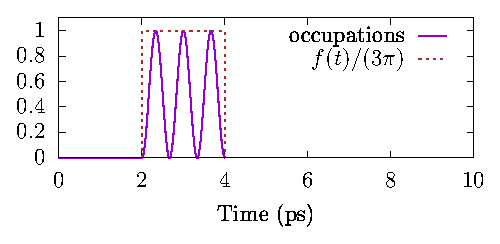
\includegraphics[width=20cm]{figs/plot_pulse_from_file.eps}


\section{Including environments}
In the following subsections, we demonstrate how environment can be included.
First of all, note that as we include multiple environment modes, the 
total environment Liouville space becomes prohibitively large 
very fast and needs to be compressed to remain tractable, 
which is the core of the ACE algorithm.
To enable compression, one has to specify a criterion. Most commonly, we
use sweeps of singular value decompositions (SVDs) and only keep the subspaces
related to singular values larger than a threshold $\epsilon \sigma_0$, where
$\sigma_0$ is the largest singular value. This is enabled in the code by
specifying a value to the paramter \texttt{threshold}. To provide small values,
the C/C++ notation for powers of ten is useful, e.g., use 
\verb+-threshold 1e-7+ in the command line to enable compression with threshold
$\epsilon =10^{-7}$. 
The smaller the
threshold, the more accurate the simulation. 
However, for very small thresholds also the calculation times as well as
the memory demands increase.
Alternatively, one can fix the maximal inner dimension of
the PT MPO by defining \verb+compress_maxk+. If both are specified, 
\verb+compress_maxk+ acts as an upper bound for the inner dimension.

In principle, all that is required to add a single mode is the environment
Hamiltonian $H_E$ including the interaction with the system and the initial
environment mode density matrix, which can be provided in the form 
of two matrix valued expressions to the \verb+add_single_mode+ parameter.
For example, 

\noindent\makebox[5cm]{\rule{7cm}{0.4pt}}
\begin{verbatim}
te          10
dt           0.01
threshold    1e-7

add_single_mode    {hbar*5* (Id_2 otimes n_3) + hbar*1.*(|0><1|_2 otimes bdagger_3 + |1><0|_2 otimes b_3)}   {|0><0|_3}


initial          {|1><1|_2}
add_Hamiltonian  { 0*Id_2 }
add_Output       {|1><1|_2}

outfile      singlemode.out 
\end{verbatim}
\noindent\makebox[5cm]{\rule{7cm}{0.4pt}}

describes the Jaynes-Cummings coupling of a two-level system with a 
bosonic mode which is detuned with respect to the two-level system energy
by a frequency $5$ in units of the system-boson coupling (which is set to 1).  
This interaction conserves the number of excitations and the dynamics will 
look like strongly detuned coherent Rabi oscillations.
Note that because $H_E$ contains the system-environment interaction, it
lives on the product Hilbert space of system and environment (system part comes
first if \verb+otimes+ is used), whereas the environment initial density
matrix lives in the bare environment Hilbert space.

Adding more modes is as simple as adding more \verb+add_single_mode+ lines
to the parameter file. However, for many practically relevant bath more 
convenient sets of command line parameters are provided, some of which 
we discuss in the following subsection.

\subsection{Fermionic environment}
One of the predefined 
environments is defined by the Fermionic hopping Hamiltonian
\begin{equation}
H_E^k=\hbar g \big( c^\dagger_k c_S + c^\dagger_S c_k ) 
+ \hbar\omega_k c^\dagger_k c_k
\end{equation}
Here, the system is a Fermionic state that may be occupied 
$|1\rangle=c_S^\dagger |0\rangle$ or not $|0\rangle$.
The occupation is created by $c^\dagger_S$ or destroyed by $c_S$. 
The environment consists of several Fermionic states, whose 
occupations are created and destroyed by $c^\dagger_k$ and $c_k$, respectively.
In the limit $N_E\to \infty$, the environment consists of a continuum of state,
which can be used to model the electronic states in metallic contacts in
proximity to a molecule or a quantum dot.
Consider the driver file:

\noindent\makebox[5cm]{\rule{7cm}{0.4pt}}
\begin{verbatim}
te                  5
dt                  1e-2
threshold           1e-7

Fermion_N_modes       2
Fermion_g             1 
Fermion_omega_min     0
Fermion_omega_max     0
Fermion_EFermi        1e4

outfile             Fermion_N2.out
\end{verbatim}
\noindent\makebox[5cm]{\rule{7cm}{0.4pt}}

\verb+Fermion_*+ indicates that what comes after is a parameter for
the Fermionic environment specified by the above Hamiltonian. 
\verb+Fermion_N_modes+ tells the code to use 2 Fermionic states as environment.
The coupling strength is determined by \verb+Fermion_g+ and the energies 
are equidistantly sampled from \verb+Fermion_omega_min+ to \verb+Fermion_omega_max+
(in inverse picoseconds; there also exist the alternative 
\verb+Fermion_E_min+ and \verb+Fermion_E_max+ to specify the band width in 
units of meV).
Here, both limits are set to zero, so that both environment modes are 
resonant to the TLS transition. By setting \verb+Fermion_EFermi 1e4+ 
the Fermi level is set to such
a high value that all environment states are initially occupied. 
There is also the parameter \verb+Fermion_temperature+ to specify the temperature
(in units of Kelvin) of the Fermi distribution. 
If not specified, the global \verb+temperature+ 
parameter will be used, whose default is 0 K.

Here, the initial state of the system is empty. Therefore, electrons will 
start to move from the Fermionic environment to the system.
The dynamics is show below and it is discussed in the ACE article.

\includegraphics[width=20cm]{figs/plot_hopping_N2.eps}


Typically, the environments of open quantum system are assumed to form 
a continuum. In ACE, we simply discretize the continuum. For the case 
of metallic leads, it turns out that using $N_E=10$ modes is already
not too bad. 
Consider the driver file \verb+Fermion.param+:

\noindent\makebox[5cm]{\rule{7cm}{0.4pt}}
\begin{verbatim}
te                  2.5
dt                  1e-2
threshold           1e-7

Fermion_N_modes      10
Fermion_rate          1 
Fermion_omega_min    -5
Fermion_omega_max     5
Fermion_EFermi        1e4

outfile             Fermion_N10.out
\end{verbatim}
\noindent\makebox[5cm]{\rule{7cm}{0.4pt}}

Here, instead of \verb+Fermion_g+, we use \verb+Fermion_rate+ to specify the 
rate that we would expect in the Markov limit. Then, the coupling constant  
is calculated internally by solving the Fermi's golden rule expression for $g$.
The respective dynamics is compared with the Markovian result
$1-\exp(-x)$ in the following plot:

\includegraphics[width=20cm]{figs/plot_hopping_N10.eps}

Increasing $N_E$ even further to about 100 while keeping the same density of 
states (i.e. increasing the band width simultaneously) will produce a behaviour
very close to the Markovian results.


\subsection{Bosonic environments}
The class of \verb+Boson_*+ environments covers environment 
Hamiltonians of the form
\begin{equation}
H_E=
\sum_{\mathbf{k}} \bigg[\hbar\omega_\mathbf{k}a^\dagger_\mathbf{k}a_\mathbf{k}
+ \hbar g_\mathbf{k}\big(a^\dagger_\mathbf{k} \hat{O}_{sys}
+a_\mathbf{k} \hat{O}_{sys}^\dagger\big) \bigg].
\end{equation}
In the case $\hat{O}_{sys}=|1><1|_2$, this leads to the independent boson model,
which is often used to model the effects of vibrational baths (phonons).
If instead $\hat{O}_{sys}=|0><1|_2$ is used, the Hamiltonian describes 
Jaynes-Cummings interactions, e.g., a quantum emitter coupled to
photon modes. This name of the parameter for this operator is 
\verb+Boson_SysOp+.

The command line arguments are similar to that for the Fermionic case, only 
that \verb+Fermion_*+ is replaced by \verb+Boson_*+.
The main differences to the Fermionic case are that initial thermal states 
now follow Bose statistics and that the number of 
excitations per mode is, in principle, unbounded. Here, we truncate the
Boson Hilbert space per mode and only account for the $M$ lowest states,
i.e. $M-1$ excitations. This information if provided to the code by the
parameter \verb+Boson_M+, whose default value is $M=2$. 

As a first example, consider the radiative decay of an initially excited
two-level quantum emitter. The corresponding parameter file 
\verb+radiative_decay.param+ is


\noindent\makebox[5cm]{\rule{7cm}{0.4pt}}
\begin{verbatim}
te                  2.5
dt                  1e-1
threshold           1e-5

Boson_N_modes       20
Boson_SysOp         {|0><1|_2}
Boson_rate           1 
Boson_omega_min    -10 
Boson_omega_max     10
Boson_temperature    0

initial             {|1><1|_2}

outfile             radiative_decay.out
\end{verbatim}
\noindent\makebox[5cm]{\rule{7cm}{0.4pt}}

The resulting dynamics resembles the Markovian result with excited state
occupations
$\langle (|1\rangle\langle 1|) \rangle= \exp(-t)$. 
(Again, an environment with larger band width would lead to a more Markovian 
behaviour, but has to be discretized with more modes and therefore takes
longer to calculate.).

One caveat for calculations at finite temperatures: The Jaynes-Cummings 
Hamiltonian acts in the rotating frame. This means that the physical energy 
of a Bosonic excitation is actually $(\hbar\omega + E_{shift}) n $, where 
$E_{shift}$ is the energy shift corresponding to the frequency of 
the rotating frame. Hence, negative values of $\omega$ are physically allowed 
if their modulus is smaller than $E_{shift}$. For initial thermal states, 
this value can be provided by \verb+Boson_E_shift_init+ or 
\verb+Boson_omega_shift_init+. The latter is internally multiplied by $\hbar$.


For structured baths where every environment mode is coupled to the system
with a different strength, i.e., $g_k$ is not constant as a function of $k$,
there are different ways to pass the values for $E_k=\hbar\omega_k$ and
$g_k$ to the code. One way is to compile a file with two columns, the first
listing the values of $E_k$ (or $\omega_k$) and the second listing 
the corresponding values of $g_k$. Please make sure the number of lines
matches \verb+Boson_N_modes+. The name of this file can be passed to the 
code by the argument \verb+Boson_E_g_from_table+ 
(or \verb+Boson_omega_g_from_table+). 
For example, if we create the file ``N20.tab'' with the 20 lines
\begin{verbatim}
-9.5   {1/sqrt(2*pi)}
-8.5   {1/sqrt(2*pi)}
-7.5   {1/sqrt(2*pi)}
-6.5   {1/sqrt(2*pi)}
...
 9.5   {1/sqrt(2*pi)}
\end{verbatim}
the following driver file
\begin{verbatim}
te                  2.5  
dt                  1e-1  
threshold           1e-5  
 
Boson_N_modes       20  
Boson_SysOp         {|0><1|_2}  
Boson_omega_g_from_table   N20.tab 
Boson_temperature    0  
 
initial             {|1><1|_2}  
 
outfile             radiative_decay_tab.out 
\end{verbatim}
exactly reproduces the results in ``radiative\_decay.out''.

Another way, which is highly recommended, is to use instead a spectral density
defined by
\begin{equation}
J(\omega)=\sum_k g_k^2 \delta(\omega-\omega_k)
\end{equation}
which is assumed to be a continuous function of $\omega$ 
in the limit of infinitely fine discretization. 
The spectral density has a more intuitive interpretation. For example, 
in the case of radiative decay, the radiative decay rate in the Markov
limit of a system driven with frequency $\omega$ is $2\pi J(\omega)$, 
a finding which we reproduce numerically next. 
In contrast, to reproduce a given rate, the values of $g_k$ have to be modified
when the discretization changes.

A spectral density can be provided to the ACE code in the form of a file that
contains two columns corresponding to a set of sample points $\omega_i$ and
$J(\omega_i)$. The sample points $\omega_i$ are not related to the 
discretization used for defining the set of environment modes. Instead, the
frequency domain from \verb+Boson_omega_min+ to \verb+Boson_omega_max+ is
discretized into \verb+Boson_N_modes+ intervals and the corresponding values
for $g_k$ are obtained by linearly interpolating between the closest sample
points to $\omega_k$ in the spectral density file. This way, the spectral 
density file has to be generated only once and can be reused for calculations
with different mode discretizations. In the following example, we reproduce 
the above result for radiative decay, now using a flat spectral density. 
To this end, generate the file \texttt{Jflat.J} with the following two lines
\begin{verbatim}
-100. 1.
 100. 1.
\end{verbatim}
Therefore, all interpolated values of $J(\omega)$ will be 1. We then 
use the parameter file
\begin{verbatim}
te                  2.5
dt                  1e-1
threshold           1e-5

Boson_N_modes       20
Boson_SysOp         {|0><1|_2}
Boson_J_from_file    Jflat.J
Boson_J_scale        {1/(2*pi)}   
Boson_omega_min    -10
Boson_omega_max     10
Boson_temperature    0

initial             {|1><1|_2}

outfile             Jflat.out
\end{verbatim}

The parameter \verb+Boson_J_scale+ rescales the spectral density by a global
factor for all sample points, in this case $1/(2\pi)$, so the expected
Markovian rate will be $2\pi J(\omega)=2\pi (1/(2 \pi))=1$. Please check 
that this approach reproduces exactly the result for radiative decay 
discussed above.


\subsection{Predefined spectral densities}

Some commonly used spectral densities are predefined and can be 
enabled by the command line argument \verb+Boson_J_type+. 
For example, one often uses spectral densities of the form 
\begin{equation}
J(\omega)=\alpha \omega^s  H(\omega),
\end{equation}
which is characterized by the exponent $s$ distinguishing ohmic $s=1$ from
sub- ($s<1$) and superohmic ($s>1$) spectral densities. $\alpha$ sets the
strength of the system-bath coupling and $H(\omega)$ is a cut-off function
used to make the large-$\omega$ limit well defined. 
This type of spectral density is activated by setting \verb+Boson_J_type+
to \verb+ohmic+.
$\alpha$ and $s$ can be set via \verb+Boson_J_alpha+ and \verb+Boson_J_s+,
respectively. The finite energy range defined by \verb+Boson_omega_min+ and
\verb+Boson_omega_max+ already leads to a natural cutoff, but one can 
also use, e.g., an exponential cutoff $H(\omega)=exp(-\omega/\omega_c)$ 
by setting \verb+Boson_J_cutoff+ to \verb+exp+ and \verb+Boson_J_omega_c+
to $\omega_c$.

Keep in mind that the generated spectral density can be printed by 
providing a file name to the parameter \verb+Boson_J_print+, which can be 
useful for debugging.

%\subsection{Phonon interactions in quantum dots}

The independent boson model, i.e, a TLS diagonally and linearly coupled 
to a continuum of harmonic oscillators, is also a good model for 
the coupling between electronic states in a quantum dot (QD) and longitudinal
acoustic phonons. The corresponding Hamiltonian is

\begin{equation}
H_E=\sum_{\mathbf{q}}\bigg[
\hbar\omega_{\mathbf{q}} b^\dagger_{\mathbf{q}}b_{\mathbf{q}}+
\hbar\gamma_{\mathbf{q}} \big( b^\dagger_{\mathbf{q}}+b_{\mathbf{q}}\big)
|X\rangle\langle X|\bigg],
\end{equation}

where $b^\dagger_{\mathbf{q}}$ and $b_{\mathbf{q}}$ are creation and
annihilation operators for phonons with wave vector $\mathbf{q}$.

Due to the ordered structure of solid state crystals, 
electron-phonon interactions are well understood and can be derived from
microscopic considerations. It turns out that the dominant 
deformation potential coupling to longitudinal acoustic phonons is 
superohmic with exponent $s=3$.
For a typical GaAs-based semiconductor quantum dot, 
a set of parameters that enter the spectral density has been worked out 
by Krummheuer \textit{et al.} in [Phys. Rev. B 71, 235329 (2005)].
To use them, simply set \verb+Boson_J_type+ to \verb+QDPhonon+.
Try the following parameter file \verb+QDPhonon_ACE.param+:

\begin{verbatim}
te                   20
dt                    1e-1
Nintermediate        20

threshold             5e-8
dict_zero             1e-12

add_Hamiltonian            {-1.5*|1><1|_2}
add_Pulse Gauss  7 5 3 0   {|1><0|_2}

Boson_N_modes                    100
Boson_M                            3
Boson_E_max                        5
Boson_J_type                       QDPhonon
Boson_subtract_polaron_shift       true
temperature                        4

outfile                            QDPhonon_ACE.out
\end{verbatim}

Two parameters in this file have not been discussed so far, 
\verb+dict_zero+ and \verb+Boson_subtract_polaron_shift+.
The former enables a trick to increase efficiency based on 
group decomposition as discussed in the supplementary material of the
ACE article on the example of superradiance, which is also related to 
[Phys. Rev. B 96, 201201(R) (2017)] describing an analogous idea for
the iQUAPI method:
For certain types of couplings, MPO matrices 
$\mathcal{Q}_{d_l d_{l-1}}^{(\alpha_l,\tilde{\alpha}_l)}$ are identical
for different combinations of $(\alpha_l,\tilde{\alpha}_l)$. 
In this case, only one representation has to be stored and calculated, which 
reduces the numerical demands. In the above example with diagonal coupling 
(\verb+Boson_SysOp+ has the default value of \verb+|1><1|_2+), the
environment does not induce system transitions, so 
$\mathcal{Q}_{d_l d_{l-1}}^{(\alpha_l,\tilde{\alpha}_l)}=0$ for 
$\alpha_l\neq\tilde{\alpha}_l$. These don't have to be stored, reducing 
the numerical demands by at least a factor of 4 ($2^2$ instead of $2^4$ 
combinations of $(\alpha_l,\tilde{\alpha}_l)$). Which matrices are zero and
which are identical with matrices for other combinations of system indices 
can be computed automatically from the microscopic Hamiltonian. 
The parameter \verb+dict_zero+ tells the code what can be considered as 
practically zero or practically identical for this purpose. If a positive
value is given, automatic detection of groups with identical couplings 
is enabled.

Setting \verb+Boson_subtract_polaron_shift+ to \verb+true+ tells the code
to subtract polaron shift from the system energy levels: 
For the independent boson model, it is well known that the 
interaction with the bath renormalizes the energies of the system
by the polaron shift 
$\Delta E_p=-\sum_{\mathbf{q}}(\gamma^2_{\mathbf{q}})/(\omega_{\mathbf{q}})
=-\int\limits_0^\infty d\omega\, J(\omega) / d\omega$.
As this shift is present irrespective of the state of the system or the 
environment, experimental determination of the energy levels of the TLS
usually reveals the polaron shifted values. It is therefore convenient to
subtract the polaron shift, redefine the energy levels, and avoid dealing 
with renormalization effects explicitly when comparing calculations with
and without phonons. 


\subsection{Related computational methods}
Finally, as an alternative to ACE, the process tensor for Gaussian baths can be 
calculated using expressions where the bath is already integrated out
[cf. {J{\o}rgensen and Pollock} Phys. Rev. Lett. 123, 240602 (2019)]. 
This method is usually much more 
efficient and does not require discretization or truncation of the phonon
Hilbert spaces (Recall: The advantage of ACE is its generality, while 
the latter method only works for Gaussian baths.)
To use this method instead for phonon simulations with our standard QD
phonon spectral density, one only needs to set \verb+use_Gaussian+ to 
\verb+true+. For example, we can re-use the parameter file from the
last example and run:

\begin{verbatim}
> ACE QDPhonon_ACE.param -use_Gaussian true -outfile QDPhonon_Gaussian.out
\end{verbatim}

With the ACE code, we also provide binaries for the iterative methods 
iQUAPI and TEMPO. If they are compiled, you can also try
\begin{verbatim}
> TEMPO QDPhonon_ACE.param -outfile QDPhonon_TEMPO.out
\end{verbatim}
or
\begin{verbatim}
> iQUAPI QDPhonon_ACE.param -n_max 12 -dt 0.2 -outfile QDPhonon_iQUAPI.out
\end{verbatim}
Note that iQUAPI performs no tensor network compression but instead 
works by memory truncation, where only a fixed maximal number
\verb+n_max+ of past time steps are accounted for.
Because the memory demands scale exponentially with \verb+n_max+, 
only relatively small values of \verb+n_max+ can be used in practice.
To cover the memory time of the environment the time step width \verb+dt+ 
should be choosen as large as possible.

\subsection{Reading, writing, and combining process tensors}

A PT generated by the ACE cod ecan be written into a binary file with a name
specified by the \verb+write_PT+ parameter. Such a PT can then be read 
for another simulation using the \verb+read_PT+. 
Furthermore, multiple PTs can be loaded and used for the propagation by the
\verb+multi_PT+ argument. The difference between the use of \verb+read_PT+ 
and \verb+multi_PT+ is that when new baths are specified, e.g., by setting 
\verb+Boson_N_modes+ or \verb+Fermion_N_modes+ to nonzero values or using 
an \verb+add_single_mode+ line, these new baths will be incorporated into
a PT specified by \verb+read_PT+, while the PTs defined by \verb+multi_PT+ 
are only loaded for the propagation of a concrete simulation.

\iffalse
analyse_PT, extend
\fi

\section{Concluding remarks}
Further developments of ACE, the method as well as the code, 
are ongoing projects. Some implemented features are not described in the 
documentation yet, but will be added in the future.

\end{document}
